\chapter{Caso Studio: Isole robotizzate di piegatura} \label{sec:CasoStudio}

In questo capitolo analizziamo la messa a punto dello SCADA su un impianto demo, nello specifico una cella di presso-piegatura robotizzata fornita da Salvagnini, uno dei maggiori clienti in Rea. Dopo aver progettato l'HMI, la fase successiva consiste nel far comunicare PLC allo SCADA attraverso l'importazione dei tag del PLC e la configurazione di questi ultimi su variabili di modello.

\section{Importazione Tag}
Per quanto riguarda l'importazione dei tag, esistono due modalità principali da seguire in FT Optix™:
\begin{enumerate}
    \item \textbf{Collegamento diretto}: Viene sfruttato il protocollo interno di FT Optix™ per stabilire una connessione diretta tra software e PLC.
    \item \textbf{Importazione da file di progetto:} Viene utilizzato un file con estensione \verb|.ap17|, generato da tecnici PLC attraverso il software \textit{Siemens TIA Portal}. Questo metodo è spesso preferito per la sua praticità, in quanto permette di lavorare con un file già configurato sulle scelte progettuali dei tecnici PLC.
\end{enumerate}
Per il nostro caso studio utilizzeremo la seconda modalità. L'intera procedura si svolge su ambiente FT Optix™, seguendo questi passaggi. In primo luogo, la configurazione avviene nella Project view, come mostrato in figura \ref{fig:ImportTag.png}, nella sezione \verb|CommDrivers|. Al suo interno viene creato un nuovo driver dalla lista di quelli supportati da FT Optix™. Nel nostro caso andremo a crearne uno di tipo \verb|S7 TIA PROFINET driver|, compatibile con il PLC Siemens utilizzato. Fatto questo, viene aggiunta una nuova Station con annesso il percorso del file \verb|.ap17|, nella sezione delle proprietà. Una volta completati i passaggi sopra descritti, da FT Optix™, dovremo selezionare la cartella contenente i tag di nostro interesse e trovarci davanti ad una struttura contente la cartella importata, con le relative variabili tag organizzate per tipologia (fare riferimento alla cartella generata in figura \ref{fig:ImportTag.png}). Questo facilita il mapping e la configurazione successiva.

\begin{figure} 
    \centering
    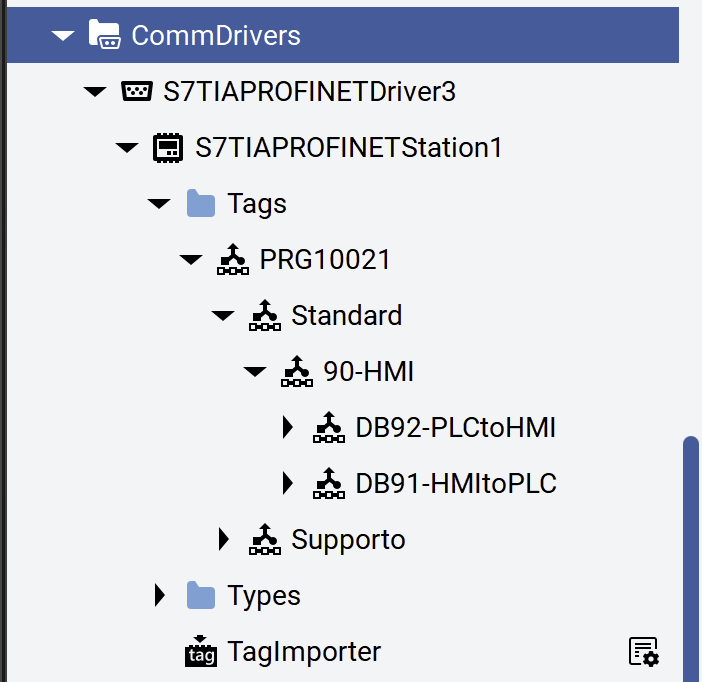
\includegraphics[width=0.4\linewidth]{Immagini/ImportTag.png}
    \caption{Illustrazione Tag importati}
    \label{fig:ImportTag.png}
\end{figure}

\section{Configurazione variabili}
Per quanto riguarda la gestione dei tag importati in precedenza, ci sono due strade da poter percorrere: lavorare direttamente sui tag importati con il rischio di avere accessi indesiderati e difficoltà nella manutenzione del sistema; oppure definire un livello di astrazione che separi i tag PLC dalle funzionalità dell'HMI. Per ovviare al problema della prima strada, adottiamo l'approccio che prevede sin da subito la creazione di variabili di modello in FT Optix™, per poi renderle intermediarie tra i tag del PLC e le funzionalità di FT Optix™. Questo approccio permette di rendere molto più sicuro l'utilizzo dell'HMI non avendo accessi diretti ai tag, e favorisce un maggior controllo dello SCADA. In secondo luogo si utilizza uno script per creare associazioni bidirezionali (\textit{dynamic links})\textsuperscript{\cite{factorytalk_setdynamiclink}} tra le variabili appena create e i tag importati dal PLC. Partiamo con il creare le variabili di modello, per cui è sufficiente creare all'interno della sezione Project view sotto la voce \verb|Model,| una cartella \verb|Drivers| in cui si definiscono tutte le variabili. Ovviamente le variabili devono essere configurate con nomi significativi per facilitare l'identificazione e l'uso. Una volta definite le variabili di modello, si passa alla parte di associazione, grazie ad un nuovo script di tipo \verb|Design-time NetLogic| in cui viene creata una funzione che comprenda la seguente struttura:
\begin{itemize}
    \item \textbf{Lista variabili di modello}: le variabili di modello sono ottenute tramite il metodo \verb|GetVariable|, specificando il path all'interno della struttura di progetto. Per ottenere il path eseguiamo gli stessi passaggi illustrati nei capitoli precedenti.
    \item \textbf{Lista dei tag PLC}: analogamente, i tag del PLC sono identificati con il loro path sotto la sezione \verb|CommDrivers|.
    \item \textbf{Creazione dynamic link}: l'associazione tra le variabili di modello e i tag del PLC avviene grazie al metodo \verb|SetDynamicLink| fornito da FT Optix™, configurato con la modalità \verb|ReadWrite| nel caso di lettura e scrittura su variabile, \verb|Read| per la lettura e \verb|Write| per la sola scrittura.
\end{itemize}
\begin{minted}[bgcolor=bgcolor, 
               linenos=true, 
               numbersep=8pt, 
               fontfamily=tt, 
               fontsize=\tiny, 
               breaklines=true, 
               breakanywhere=true]{csharp}
...

public class AssociazioneVarModelloAPLC : BaseNetLogic
{
    [ExportMethod]
    public void Method1()
    {
        /*------------------------------------------------
          variabili di modello 
        */
        
        //DB91
        var modello000 = Project.Current.GetVariable("Model/Drivers/DB91/DB91_CambioProduzione");
        ... // la lista prosegue con tutte le variabili di modello

        /*------------------------------------------------
          variabili di PLC
        */

        // DB91
        var varPLC000 = Project.Current.GetVariable("CommDrivers/S7TIAPROFINETDriver3/S7TIAPROFINETStation1/Tags/PRG10021/Standard/90-HMI/DB91-HMItoPLC/CambioProduzione");
        ... // la lista prosegue con tutte le variabili di PLC

        /*------------------------------------------------
          dynamicLink per Optix
        */
        modello000.SetDynamicLink(varPLC000, DynamicLinkMode.ReadWrite);
        ... // la lista prosegue con tutti i dynamicLink tra la prima e seconda lista
        
        }
}
\end{minted}
Questa modalità ha molteplici vantaggi. Prima di tutto, la sicurezza è migliorata: l'astrazione evita che l'HMI interagisca direttamente con i tag del PLC, e permette di impostare la modalità in lettura e/o scrittura, che riduce significativamente il rischio di accesso non autorizzato. Inoltre, la manutenzione viene semplificata: la separazione tra modello e tag facilita eventuali modifiche future al sistema ed un eventuale reimpiego dell'HMI. Infine, la scalabilità: l’utilizzo di uno script per la configurazione consente di gestire facilmente un numero elevato di variabili e tag direttamente in un unica funzione. Nonostante i numerosi vantaggi offerti da questo approccio, è importante evidenziare alcune criticità operative legate a sistemi complessi con migliaia di variabili. Più nello specifico: nei sistemi con elevato numero di variabili, il processo di messa a punto diventa un'operazione altamente dispendiosa in termini di tempo. Ciò accade perché ogni variabile di modello viene associata al corrispondente tag PLC tramite script. Una soluzione plausibile per sistemi avanzati potrebbe essere di automatizzare lo script di configurazione tramite il mapping delle variabili.

\subsection{Gestione FTP Robot, FTP Pressa e passi 50, 55 e 60}
Nei \verb|case 50, 55 e 60| citati in precedenza, vengono gestiti tutti i caricamenti dei programmi, sia della pressa piegatrice, sia del robot dell'impianto. Per richiesta, è stato scelto sin dall'inizio di gestire entrambi i programmi dal lato interfaccia, con la seguente lettura dei dati tramite macchina a stati. Partendo dalla progettazione HMI, entrambi i pannelli sono stati inseriti nella sezione impostazioni, con accesso riservato solo agli utenti con autorizzazione appropriata, come in figura \ref{fig:FTP.png}.
\begin{figure} [ht]
    \centering
    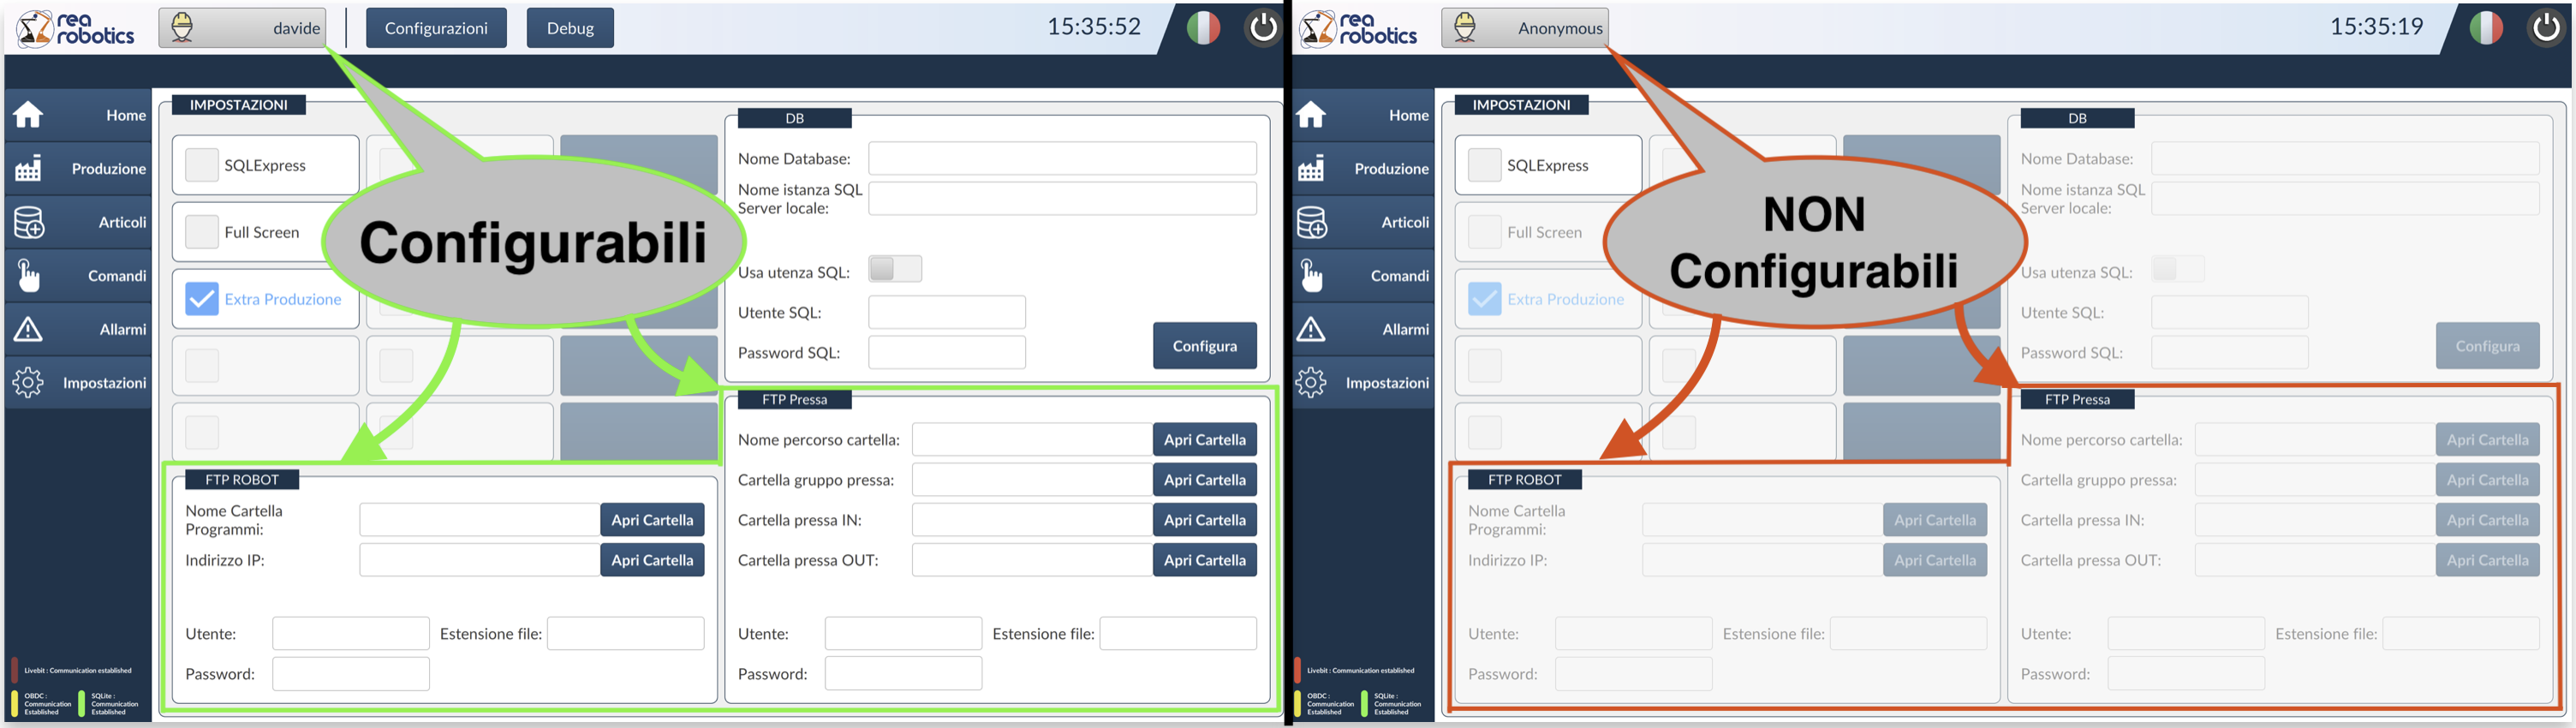
\includegraphics[width=\linewidth]{Immagini/FTP.png}
    \caption{Illustrazioni Gestione FTP Robot ed FTP Pressa}
    \label{fig:FTP.png}
\end{figure}

Entrando nello specifico, in questa sezione sono stati inseriti 2 pannelli che rispettassero i seguenti requisiti:
\begin{enumerate}
    \item \textbf{FTP Robot:} in cui è permesso selezionare il nome della cartella contenente i programmi robot, con estensione ed altri parametri specifici dell'impianto.
    \item \textbf{FTP Pressa:} richiede informazioni più dettagliate, tra cui le cartelle di input ed output del programma, oltre al nome specifico per la pressa e le credenziali di rete per un eventuale gestione tramite FTP.
\end{enumerate}
Queste due sezioni sono fondamentali per poter riuscire a far comprendere all'impianto che tipo di istruzioni debba eseguire la macchina (robot e/o pressa) durante il caricamento di un ordine di produzione. I file contenenti le istruzioni del robot e quelli per la pressa vengono prodotti rispettivamente da chi si occupa della gestione robot e della gestione pressa. Per quanto riguarda, invece, la lettura tramite macchina stati, i passi da analizzare sono il 50, 55 e 60:
\begin{itemize}
    \item \verb|case 50|: in questo passo, il sistema si trova in attesa della richiesta da parte del PLC del caricamento del programma. Una volta ricevuta, in caso affermativo il sistema passa al passo 55; in caso di KO invece il passo viene impostato a 180.
    \item \verb|case 55|: il sistema esegue una serie di operazioni in cui vengono lanciate le funzioni di gestione programma, con annesso controllo dell'esistenza del file nel percorso indicato, copia del file dalla sorgente alla destinazione e verifica della consistenza del file copiato. Inoltre, ogni funzione ha una gestione degli errori con popup adeguati, restituendo valori in base all'esito (questa parte è presente in \verb|script_maincycle.cs|). Se tutto avviene in modo corretto, si passa al passo 60.
    \item \verb|case 60|: seconda ed ultima fase di attesa da parte dell'HMI nei confronti del PLC. Più nello specifico, l'HMI verifica che la variabile di richiesta caricamento programma desiderato sia resettata dal PLC, ed in base al risultato di questa verifica, il sistema decide quali saranno i prossimi passi da eseguire.
\end{itemize}
Quello che abbiamo analizzato in questo capitolo è la minima parte di tutto il lavoro che compone la gestione dei robot e di altri vari componenti presenti in un impianto; nel nostro caso la gestione era di due sole macchine con istruzioni ben definite. In contesti industriali più complessi, dove sono coinvolti numerosi apparati e macchine, la gestione può risultare molto più articolata e richiede soluzioni più sofisticate per garantire scalabilità, sincronizzazione e gestione di malfunzionamenti.

\begin{figure} [ht]
    \centering
    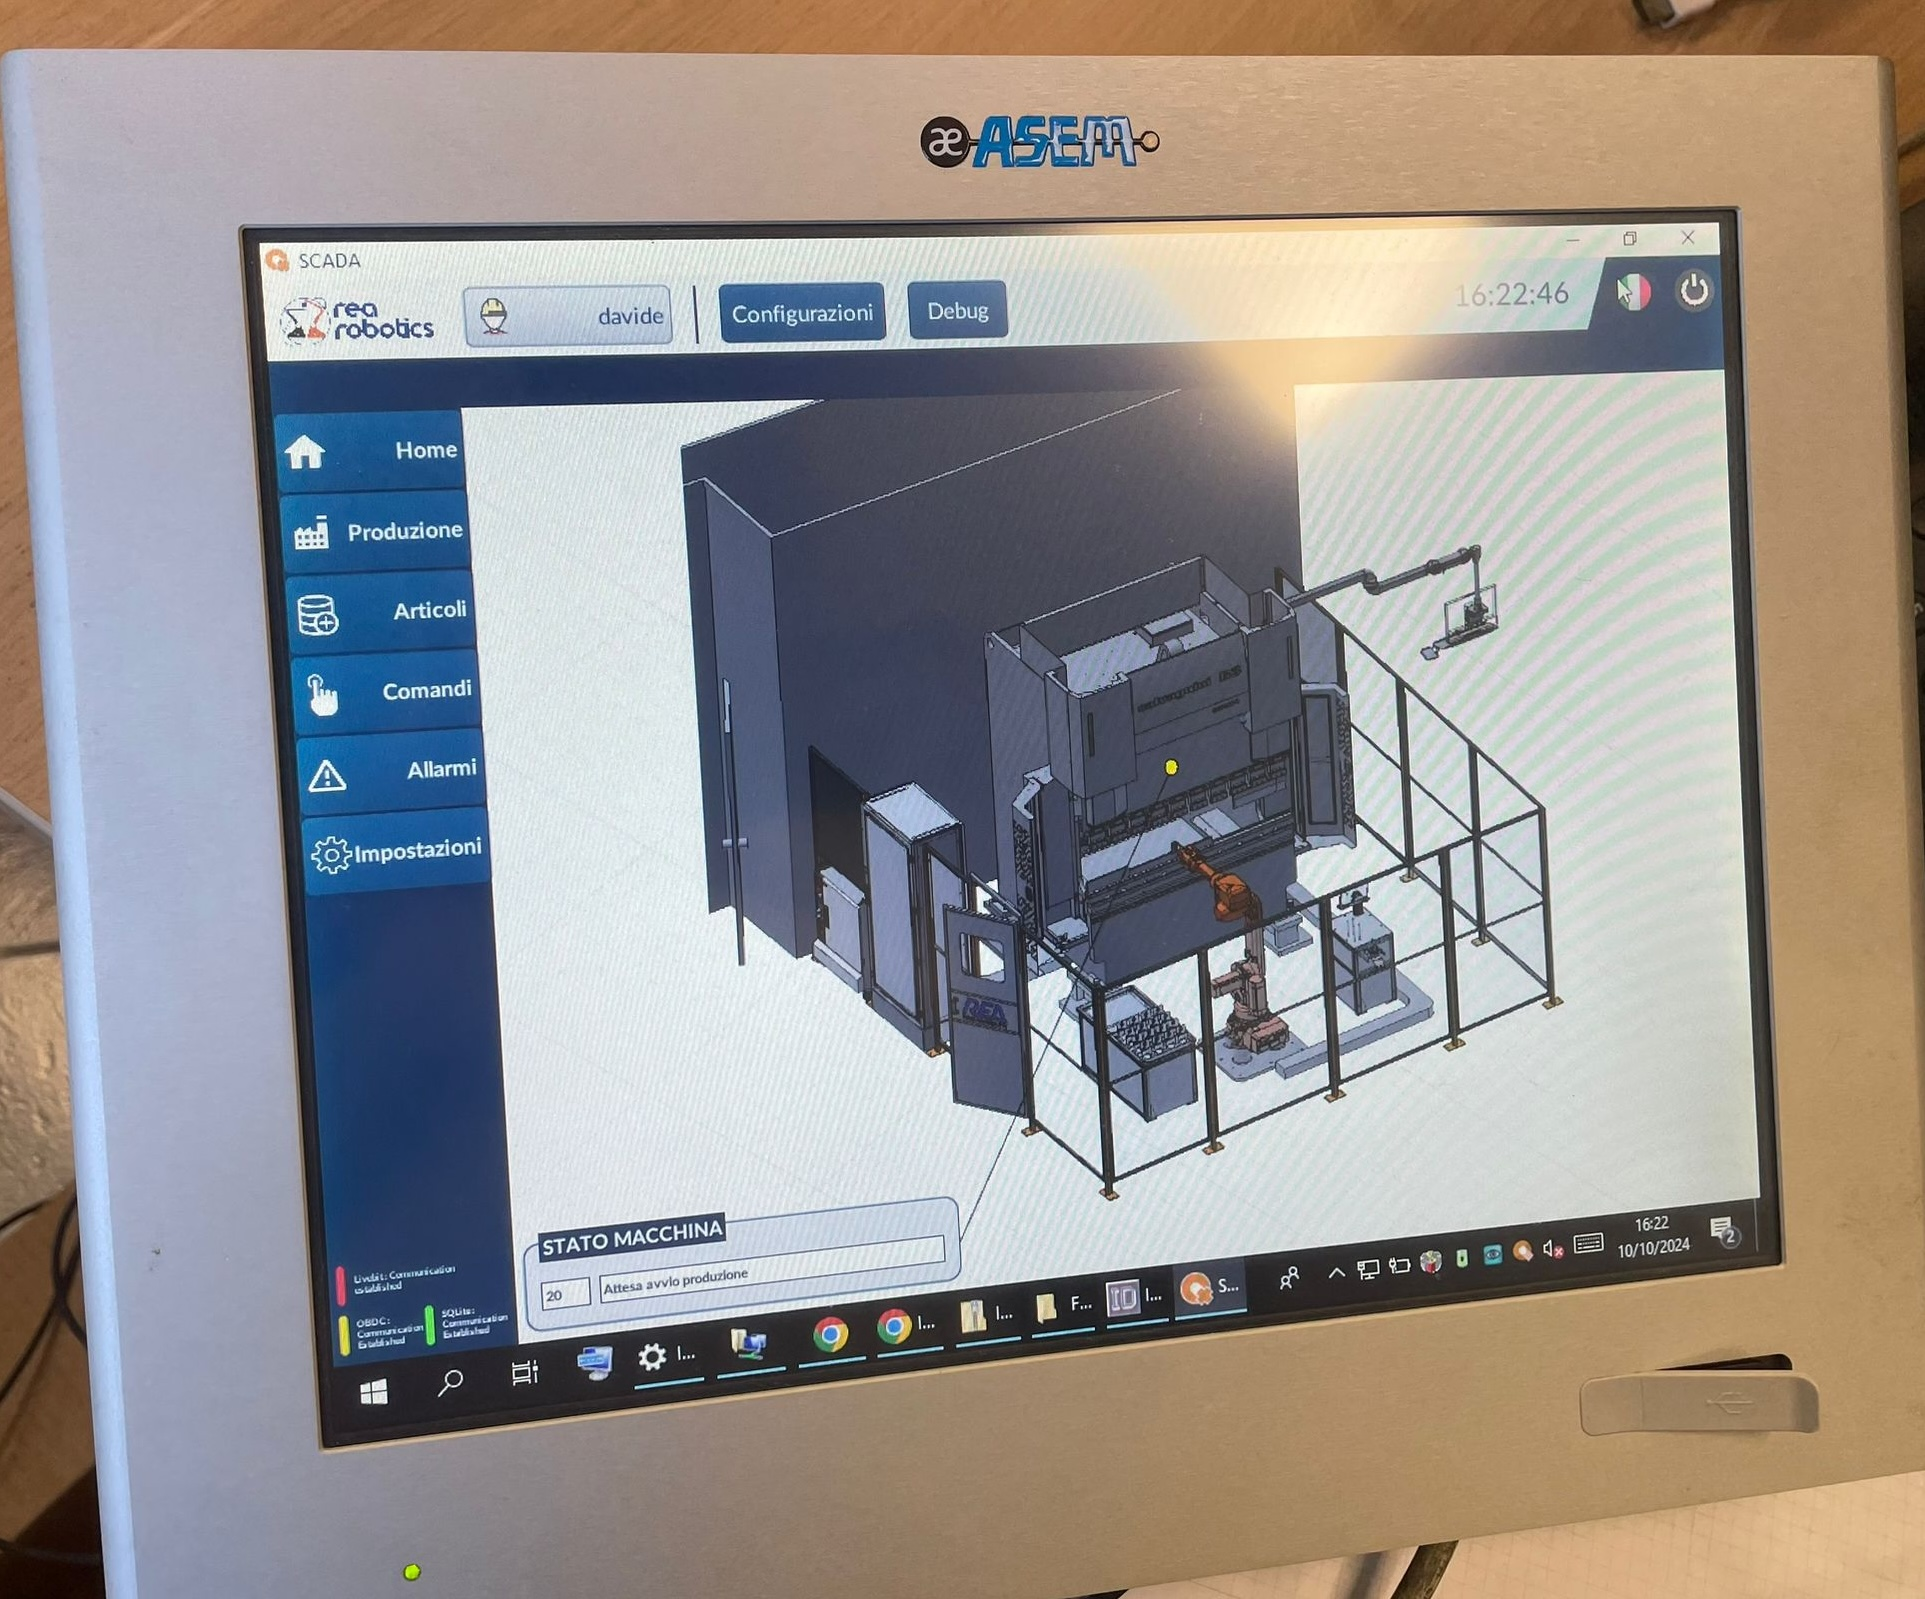
\includegraphics[width=0.7\linewidth]{Immagini/PannelloASEM.jpg}
    \caption{Prova messa in funzione dello SCADA su pannello prova ASEM}
    \label{fig:PannelloASEM.jpg}
\end{figure}